\documentclass[11pt, a4paper]{article} \usepackage{geometry} % margins + paper size
\usepackage{titlesec} % styling sections
\usepackage[fixed]{fontawesome5} % nice icons
\usepackage[svgnames]{xcolor} % color names
\usepackage{hyperref}  % for hyperlinks
\usepackage{graphicx}  % for the photo

% styling parameters >>> Configure page margins with geometry
\geometry{left=1.4cm, top=1cm, right=1.4cm, bottom=1.2cm, footskip=0.5cm}
\hypersetup{
  colorlinks=true,
  allcolors={NavyBlue}
}

\titleformat{\section}{\normalfont\Large\bfseries}{\thesection}{1em}{}[{\titlerule[0.3pt]}]
\titlespacing*{\section}{0pt}{0pt}{10pt}
\pagenumbering{gobble}
% <<<

% some formatting macros
\newcommand{\edu}[3]{
  \noindent\textbf{#1}\hfill #2\\
  #3\vspace{0.7em}}

\newcommand{\jobl}[5]{%
  \textbf{#1}\hfill #2\\
  #3\vspace{0.25em}\\
  Roles: #4\\
  Focus: #5}

\newcommand{\job}[5]{%
  \jobl{#1}{#2}{#3}{#4}{#5}\vspace{0.5em}
}

% fancy hyperlinks to external resources.
\newcommand{\mhref}[1]{\hfill\href{#1}{\small (more\faExternalLink*)}}

\begin{document}
% info header >>>
\noindent
  \begin{minipage}{0.75\linewidth}
    \strut\vspace*{-\baselineskip}\newline
    \begin{center}
    {\LARGE Curriculum Vitae\\\vspace{0.5em}\textbf{Alexey Bochkarev}}\\
    ---
    \end{center}

    \begin{minipage}{0.30\textwidth}
      \textbf{Contact:}\\
      \faEnvelope \href{mailto:a@bochkarev.io}{a@bochkarev.io}\\
      \faTelegram \href{https://t.me/abochka}{@abochka}\\
      \faPhone \textit{(phone no.)}\\
    \end{minipage}\hfill%
    \begin{minipage}{0.30\textwidth}
      \textbf{Web presence:}\\
      \faGlobe \href{https://www.bochkarev.io}{www.bochkarev.io}\\
      \faGithub \href{https://github.com/alex-bochkarev}{alex-bochkarev}\\
      \faTwitter \href{https://twitter.com/a_bochka}{@a\_bochka}\\
    \end{minipage}\hfill%
    \begin{minipage}{0.33\textwidth}
      \textbf{Personal info:} \\
      Born \textit{(when)} in \textit{(where)}\\
      (\textit{more details})\\\textit{(Nationality)}\\
      (\textit{Marital status, kids}).
    \end{minipage}
  \end{minipage}\hfill%
  \begin{minipage}{0.22\linewidth}
    \strut\vspace*{-\baselineskip}\newline
    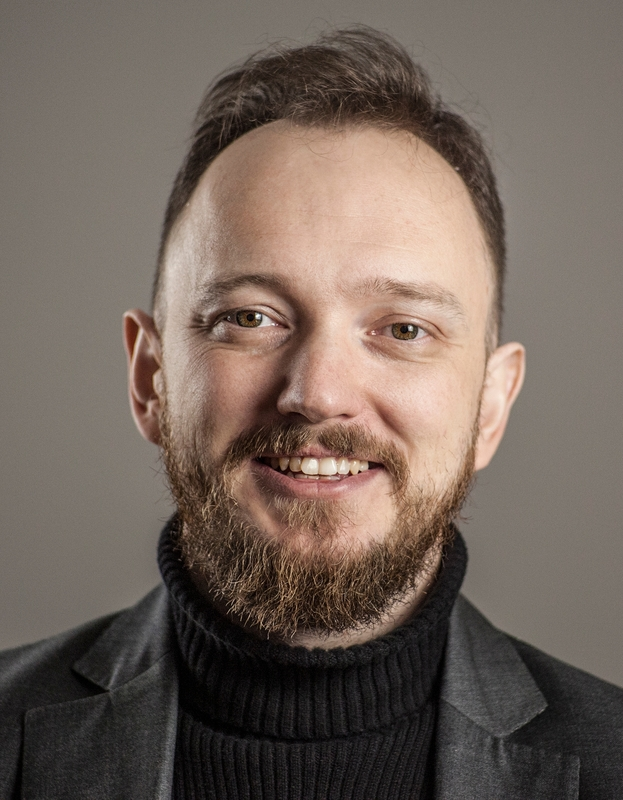
\includegraphics[width=\textwidth]{Bochkarev.jpg}
  \end{minipage}
% <<< end info header

  \vspace{1.0em}

  \section*{Education}
  \edu{PhD in Industrial Engineering}{2018--2021}{
    Clemson University, SC, USA\\
    Operations Research track}

  \noindent Dissertation: ``Selected Topics in Network Optimization: Aligning
  Binary Decision\\ Diagrams for a Facility Location Problem and a Search Method
  for Dynamic\\Shortest Path Interdiction.''
  \noindent (\href{https://tigerprints.clemson.edu/all_dissertations/2915}{https://tigerprints.clemson.edu/all\_dissertations/2915})\\
  Supervisor:
  \href{https://scholar.google.com/citations?user=87CaUHYAAAAJ&hl=en}{Dr. J.
    Cole Smith.}\vspace{1.5em}

  \edu{MA in Economics}{2008--2010}{
    New Economic School, Russia}

  \edu{MSc and BSc in Applied Mathematics and Physics}{2004--2010}{
    Moscow Institute of Physics and Technology, Russia}

  \section*{Work experience}
  \job{Clemson University}{2018--2021}{Research and teaching. Clemson, SC,
    USA}{Graduate Assistant.}{Research in Mathematical Optimization. Teaching
    assistantship in Probability Theory.}

  \noindent
  \job{Electric energy / The Federal Grid (FGC UES)}{2013--2017}{Electricity transmission.
    Moscow, Russia}{Team deputy head $\rightarrow$ Team head. Modeling and analytics}{Performance
    benchmarking (branches), operational efficiency improvement.\\ Internal
    and external regulations / KPI, strategy, analytics / modeling, and presentations.}

  \noindent
  \job{Roland Berger Strategy Consultants GmbH}{2010--2013}{Strategic consulting.
    Moscow, Russia}{Intern $\rightarrow$ Junior
    Consultant $\rightarrow$ Consultant.}{Infrastructure and construction.
    Strategy and performance: market entry,\\ supply/demand modeling, growth
    strategy, efficiency improvement. Internal knowledge sharing,\\modeling, presentations.}

  \section*{Research experience and outputs \mhref{https://www.bochkarev.io/research/}}
  Current research focus: combinatorial optimization, network optimization and
  interdiction, decision diagrams and dynamic programming, applications of
  reinforcement learning techniques. Current projects involve design and
  implementation of an algorithm and the related computational experiments.

  \begin{itemize}
    \itemsep0pt
  \item \textbf{Align-BDD:} seeking to obtain computational benefits and
    sensitivity information by representing a combinatorial problem as a
    collection of Binary Decision Diagrams (BDDs). The project involves creating a heuristic to enforce a
    certain structural property for a pair of BDDs and building a related
    computational pipeline for a specific, hard optimization problem: a
    variant of the facility location.
  \item \textbf{DSPI:} applying game-playing and reinforcement
    learning techniques to the Dynamic Shortest-path Interdiction problem,
    in a framework of a Monte-Carlo Search Tree based algorithm.
  \end{itemize}

 \subsection*{Working papers}
 \begin{itemize}
    \itemsep0pt
    \item \underline{A. A. Bochkarev}, J.C. Smith, On Aligning
    Non-Order-Associated Binary Decision Diagrams, under review in
    \textit{INFORMS Journal on Computing}. Preprint: \href{https://optimization-online.org/2022/08/on-aligning-non-order-associated-binary-decision-diagrams/}{https://optimization-online.org/2022/08/on-aligning-non-order-associated-binary-decision-diagrams/}
  \item \underline{A. A. Bochkarev}, J.C. Smith, A Monte Carlo Tree Search for
    Dynamic Shortest-Path Interdiction, under review in \textit{Networks}.
 \end{itemize}

 \subsection*{Talks}
 \begin{itemize}
   \itemsep0pt
 \item A Monte Carlo Tree Search for Dynamic Shortest-Path Interdiction,\\
   \textit{International Network Optimization Conference, 2022}, Aachen,
   Germany
   (\href{https://sites.google.com/view/inoc2022/schedule}{INOC-2022}).\hfill 2022
 \item On Aligning Non-Order-Associated Binary Decision Diagrams,\\\textit{INFORMS Annual
     Meeting, 2020} (virtual), BDD section.\hfill 2020
 \end{itemize}

 \subsection*{Grants and fellowships}
 \begin{itemize}
 \itemsep0pt
    \item Clemson University Doctoral Disseration Completion grant \hfill 2021
    \item The Seth Bonder Foundation grant (for INFORMS Annual Meeting)\hfill
      2021
    \item International Teaching Fellowship from Clemson University \hfill 2020, 2021
 \end{itemize}

 \section*{Service and volunteering.\mhref{https://www.bochkarev.io/teaching/}}
   \begin{itemize}
      \itemsep0pt
    \item Design and delivery of single lectures and mini-courses for gifted
      high-school students/undergraduates, for Puschino Winter School
      (ZPSh) and School for Molecular and Theoretical Biology (SMTB):
      \begin{itemize}
        \itemsep0pt
        \item ``Practical Introduction to Probability Theory'' \hfill 2021
        \item ``A Glimpse into Algorithms'' \hfill 2020, 2021, 2022
        \item ``How to teach machines: simple examples on ML''\hfill 2022
      \end{itemize}
      \item Clemson University INFORMS Student Chapter (Secretary, President) \hfill 2020, 2021
      \item ``Journal club on Network optimization and interdiction'' (organization) \hfill 2021
      \item ``OR Tech Seminar'' -- a series of four workshops on research
        toolbox (design and delivery) \hfill 2021
\end{itemize}

\section*{Other skills. \mhref{https://www.bochkarev.io/notes/stack}}
\begin{itemize}
  \item Main programming stack:
    \begin{itemize}
      \itemsep0pt
      \item Python (gurobi, CBC, numpy/pandas, etc.)
      \item R (ggplot, dplyr, tidyverse),
      \item Julia (JuMP/gurobi, LightGraphs),
      \item C++ (gurobi, armadillo/BLAS, boost),
      \item basic PyTorch, Java, Matlab/Octave.
    \end{itemize}
  \item Other tools: PBS (comp cluster), GNU/Linux, bash; make, git, \LaTeX,
    Emacs, basic GIS (QGIS), Inkscape, beamer / PowerPoint / reveal.js, Jupyter.
  \item (Human) languages: English (fluent), Russian (native), German ($\sim$ A1).
  \end{itemize}

   {%%% footer
   \vfill\noindent\tiny\LaTeX{}
   source: \href{https://github.com/alex-bochkarev/AB-CV}{Github}\hfill
   Updated: 2022-10-17 (\textit{Lebenslauf})}
\end{document}
